%------------------------------------------------------------------------------
%%
%------------------------------------------------------------------------------

\begin{frame}[fragile]{Marginalization}

\centering

{\footnotesize
  \only<1>{
    We marginalize each variable of interest from a sepset or cluster that contains it.
  }
  \only<2>{
    Suppose we are interested in variables $A$, $B$, and $C$.
  }
  \only<3>{
    To marginalize a variable from a \textit{cluster} we perform a product between the
    incoming messages and the cluster potential, and sum out all other variables.
  }
  \only<4>{
    To marginalize a variable from a \textit{sepset} we perform a product between the
    two messages incoming messages and sum out all other variables.
  }
}

\begin{figure}
\scalebox{0.85}{
\begin{tikzpicture}[>=latex]

  % The various elements are conveniently placed using a matrix:
  \matrix[row sep=1.00cm,column sep=1.00cm, ampersand replacement = \&] {
    % First line
                                                               \&
                                                               \&
    \node (bd) [bag,thick,minimum size=1.5cm] {$\{B,D\}$};     \&
                                                               \&
                                                              \\
    % Second line
                                                               \&
                                                               \&
    \node (b) [hsepset,thick] {$\{B\}$};                             \&
                                                               \&
                                                              \\
    % Third line
    \node (abc) [bag,thick,minimum size=1.5cm] {$\{A,B,C\}$};  \&
    \node (bc) [vsepset,thick] {$\{B,C\}$};                          \&
    \node (bce) [bag,thick,minimum size=1.5cm] {$\{B,C,E\}$};  \&
    \node (be) [vsepset,thick] {$\{B,E\}$};                          \&
    \node (bef) [bag,thick,minimum size=1.5cm] {$\{B,E,F\}$};
                                                              \\
  };

  % The diagram elements are now connected through lines:
  \path[-]
    (bd) edge (b)
    (b) edge (bce)
    (abc) edge (bc)
    (bc) edge (bce)
    (bce) edge (be)
    (be) edge (bef)
    ;

  \msgcircle{left}{down}{bd}{b}{0.6}{$1$}{MaterialBlue};
  \msgcircle{up}{left}{bef}{be}{0.6}{$2$}{MaterialBlue};
  \msgcircle{up}{left}{bce}{bc}{0.6}{$3$}{MaterialBlue};
  \msgcircle{down}{right}{abc}{bc}{0.6}{$4$}{MaterialRed};
  \msgcircle{right}{up}{bce}{b}{0.6}{$5$}{MaterialRed};
  \msgcircle{down}{right}{bce}{be}{0.6}{$6$}{MaterialRed};
    
\end{tikzpicture}

}
\end{figure}
\end{frame}

%------------------------------------------------------------------------------
%%
%------------------------------------------------------------------------------

\begin{frame}[fragile]{Marginalization}

\centering

\begin{figure}[t]
  \begin{subfigure}{4.6cm}
    \[ p(A, \bm{E=e}) = \sum_{B,C} \psi_{\bm{\{A,B,C\}}} \times \]
  \end{subfigure}
  \begin{subfigure}{0.8cm}
    \hspace{-0.5cm}
    \vspace{-0.4cm}
    \resizebox{\textwidth}{!}{
      \begin{tikzpicture}
        \msgcircle{up}{left}{a}{b}{0.0}{$3$}{MaterialBlue};
      \end{tikzpicture}
    }
  \end{subfigure}
\end{figure}

\begin{figure}
\scalebox{0.85}{
\begin{tikzpicture}[>=latex]

  % The various elements are conveniently placed using a matrix:
  \matrix[row sep=1.00cm,column sep=1.00cm, ampersand replacement = \&] {
    % First line
                                                                    \&
                                                                    \&
    \node (bd) [bag,thick,minimum size=1.5cm,mygray] {$\{B,D\}$};     \&
                                                                    \&
                                                                   \\
    % Second line
                                                                    \&
                                                                    \&
    \node (b) [hsepset,thick,mygray] {$\{B\}$};                             \&
                                                                    \&
                                                                   \\
    % Third line
    \node (abc) [bag,thick,minimum size=1.5cm] {$\{A,B,C\}$};       \&
    \node (bc) [vsepset,thick,mygray] {$\{B,C\}$};                          \&
    \node (bce) [bag,thick,minimum size=1.5cm,mygray] {$\{B,C,E\}$};  \&
    \node (be) [vsepset,thick,mygray] {$\{B,E\}$};                          \&
    \node (bef) [bag,thick,minimum size=1.5cm,mygray] {$\{B,E,F\}$};
                                                                   \\
  };

  % The diagram elements are now connected through lines:
  \path[-]
    (bd) edge[mygray] (b)
    (b) edge[mygray] (bce)
    (abc) edge[mygray] (bc)
    (bc) edge[mygray] (bce)
    (bce) edge[mygray] (be)
    (be) edge[mygray] (bef)
    ;

  \msgcircle{left}{down}{bd}{b}{0.6}{$1$}{mygray};
  \msgcircle{up}{left}{bef}{be}{0.6}{$2$}{mygray};
  \msgcircle{up}{left}{bce}{bc}{0.6}{$3$}{MaterialBlue};
  \msgcircle{down}{right}{abc}{bc}{0.6}{$4$}{mygray};
  \msgcircle{right}{up}{bce}{b}{0.6}{$5$}{mygray};
  \msgcircle{down}{right}{bce}{be}{0.6}{$6$}{mygray};
    
\end{tikzpicture}

}
\end{figure}
\end{frame}

%------------------------------------------------------------------------------
%%
%------------------------------------------------------------------------------

\begin{frame}[fragile]{Marginalization}

\centering

\begin{figure}[t]
  \begin{subfigure}{2.5cm}
    $ p(B, \bm{E=e}) =$
  \end{subfigure}
  \begin{subfigure}{0.8cm}
    \hspace{-0.3cm}
    %\vspace{-0.1cm}
    \resizebox{\textwidth}{!}{
      
\begin{tikzpicture}
        \msgcircle{left}{down}{bd}{b}{0.65}{$1$}{MaterialBlue};
      \end{tikzpicture}
    }
  \end{subfigure}
  \begin{subfigure}{0.5cm}
    \hspace{-0.55cm}
    $ \times $
  \end{subfigure}
  \begin{subfigure}{0.8cm}
    \hspace{-1.0cm}
    %\vspace{-0.1cm}
    \resizebox{\textwidth}{!}{
      
\begin{tikzpicture}
        \msgcircle{right}{up}{bce}{b}{0.65}{$5$}{MaterialRed};
      \end{tikzpicture}
    }
  \end{subfigure}
\end{figure}

\begin{figure}
\scalebox{0.85}{
\begin{tikzpicture}[>=latex]

  % The various elements are conveniently placed using a matrix:
  \matrix[row sep=1.00cm,column sep=1.00cm, ampersand replacement = \&] {
    % First line
                                                                    \&
                                                                    \&
    \node (bd) [bag,thick,minimum size=1.5cm,mygray] {$\{B,D\}$};     \&
                                                                    \&
                                                                   \\
    % Second line
                                                                    \&
                                                                    \&
    \node (b) [hsepset,thick] {$\{B\}$};                                  \&
                                                                    \&
                                                                   \\
    % Third line
    \node (abc) [bag,thick,minimum size=1.5cm,mygray] {$\{A,B,C\}$};  \&
    \node (bc) [vsepset,thick,mygray] {$\{B,C\}$};                          \&
    \node (bce) [bag,thick,minimum size=1.5cm,mygray] {$\{B,C,E\}$};  \&
    \node (be) [vsepset,thick,mygray] {$\{B,E\}$};                          \&
    \node (bef) [bag,thick,minimum size=1.5cm,mygray] {$\{B,E,F\}$};
                                                                   \\
  };

  % The diagram elements are now connected through lines:
  \path[-]
    (bd) edge[mygray] (b)
    (b) edge[mygray] (bce)
    (abc) edge[mygray] (bc)
    (bc) edge[mygray] (bce)
    (bce) edge[mygray] (be)
    (be) edge[mygray] (bef)
    ;

  \msgcircle{left}{down}{bd}{b}{0.6}{$1$}{MaterialBlue};
  \msgcircle{up}{left}{bef}{be}{0.6}{$2$}{mygray};
  \msgcircle{up}{left}{bce}{bc}{0.6}{$3$}{mygray};
  \msgcircle{down}{right}{abc}{bc}{0.6}{$4$}{mygray};
  \msgcircle{right}{up}{bce}{b}{0.6}{$5$}{MaterialRed};
  \msgcircle{down}{right}{bce}{be}{0.6}{$6$}{mygray};
    
\end{tikzpicture}

}
\end{figure}
\end{frame}

%------------------------------------------------------------------------------
%%
%------------------------------------------------------------------------------

\begin{frame}[fragile]{Marginalization}

\centering

\begin{figure}[t]
  \begin{subfigure}{2.90cm}
    \[ p(C, \bm{E=e}) = \sum_{B} \]
  \end{subfigure}
  \begin{subfigure}{0.8cm}
    \hspace{-0.25cm}
    \vspace{-0.1cm}
    \resizebox{\textwidth}{!}{
      
\begin{tikzpicture}
        \msgcircle{down}{right}{abc}{bc}{0.6}{$4$}{MaterialRed};
      \end{tikzpicture}
    }
  \end{subfigure}
  \begin{subfigure}{0.5cm}
    \hspace{-0.45cm}
    \vspace{-0.2cm}
    $ \times $
  \end{subfigure}
  \begin{subfigure}{0.8cm}
    \hspace{-0.85cm}
    \vspace{-0.4cm}
    \resizebox{\textwidth}{!}{
      \begin{tikzpicture}
        \msgcircle{up}{left}{bce}{bc}{0.6}{$3$}{MaterialBlue};
      \end{tikzpicture}
    }
  \end{subfigure}
\end{figure}

\begin{figure}
\scalebox{0.85}{
\begin{tikzpicture}[>=latex]

  % The various elements are conveniently placed using a matrix:
  \matrix[row sep=1.00cm,column sep=1.00cm, ampersand replacement = \&] {
    % First line
                                                                    \&
                                                                    \&
    \node (bd) [bag,thick,minimum size=1.5cm,mygray] {$\{B,D\}$};     \&
                                                                    \&
                                                                   \\
    % Second line
                                                                    \&
                                                                    \&
    \node (b) [hsepset,thick,mygray] {$\{B\}$};                                  \&
                                                                    \&
                                                                   \\
    % Third line
    \node (abc) [bag,thick,minimum size=1.5cm,mygray] {$\{A,B,C\}$};  \&
    \node (bc) [vsepset,thick] {$\{B,C\}$};                          \&
    \node (bce) [bag,thick,minimum size=1.5cm,mygray] {$\{B,C,E\}$};  \&
    \node (be) [vsepset,thick,mygray] {$\{B,E\}$};                          \&
    \node (bef) [bag,thick,minimum size=1.5cm,mygray] {$\{B,E,F\}$};
                                                                   \\
  };

  % The diagram elements are now connected through lines:
  \path[-]
    (bd) edge[mygray] (b)
    (b) edge[mygray] (bce)
    (abc) edge[mygray] (bc)
    (bc) edge[mygray] (bce)
    (bce) edge[mygray] (be)
    (be) edge[mygray] (bef)
    ;

  \msgcircle{left}{down}{bd}{b}{0.6}{$1$}{mygray};
  \msgcircle{up}{left}{bef}{be}{0.6}{$2$}{mygray};
  \msgcircle{up}{left}{bce}{bc}{0.6}{$3$}{MaterialBlue};
  \msgcircle{down}{right}{abc}{bc}{0.6}{$4$}{MaterialRed};
  \msgcircle{right}{up}{bce}{b}{0.6}{$5$}{mygray};
  \msgcircle{down}{right}{bce}{be}{0.6}{$6$}{mygray};
    
\end{tikzpicture}

}
\end{figure}
\end{frame}

